\documentclass[border={-4pt -6pt -4pt -4pt}]{standalone}

\usepackage{hyperref}
\usepackage{tikz}

\usetikzlibrary{decorations.pathreplacing,
  arrows,
  calc,
  decorations.pathmorphing,
  decorations.pathreplacing,
  decorations.markings,
  fadings,
  positioning,
  shapes,
  3d
}

\ifpdf
% Ensure reproducible output
\pdfinfoomitdate=1
\pdfsuppressptexinfo=-1
\pdftrailerid{}
\hypersetup{
  pdfcreator={},
  pdfproducer={}
}
\fi

\begin{document}
\begin{tikzpicture}
  \node at (0.0, 0) {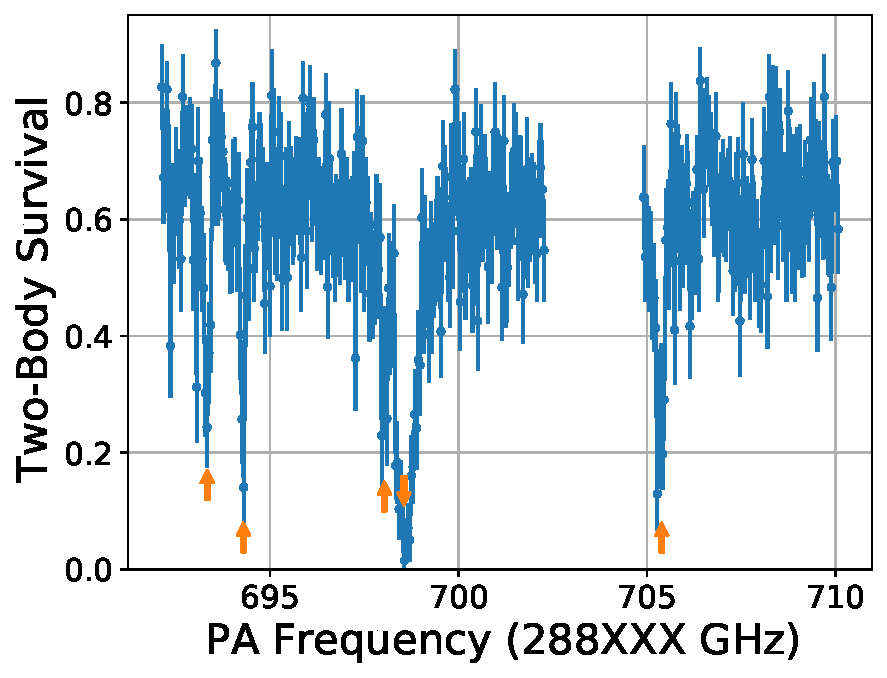
\includegraphics[height=4.5cm]{pa_spectrum_v0.pdf}};
  \node at (2.6, 1.98) {\scriptsize (\textbf{A})};
  \node at (6, 0) {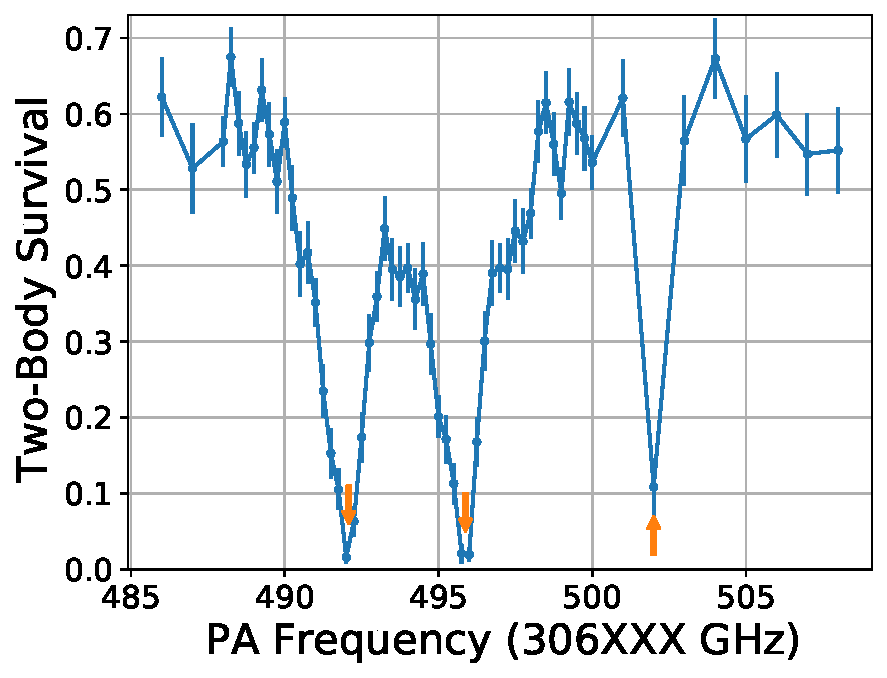
\includegraphics[height=4.5cm]{pa_spectrum_v12.pdf}};
  \node at (8.6, 1.98) {\scriptsize (\textbf{B})};
  \node at (0.0, -4.6) {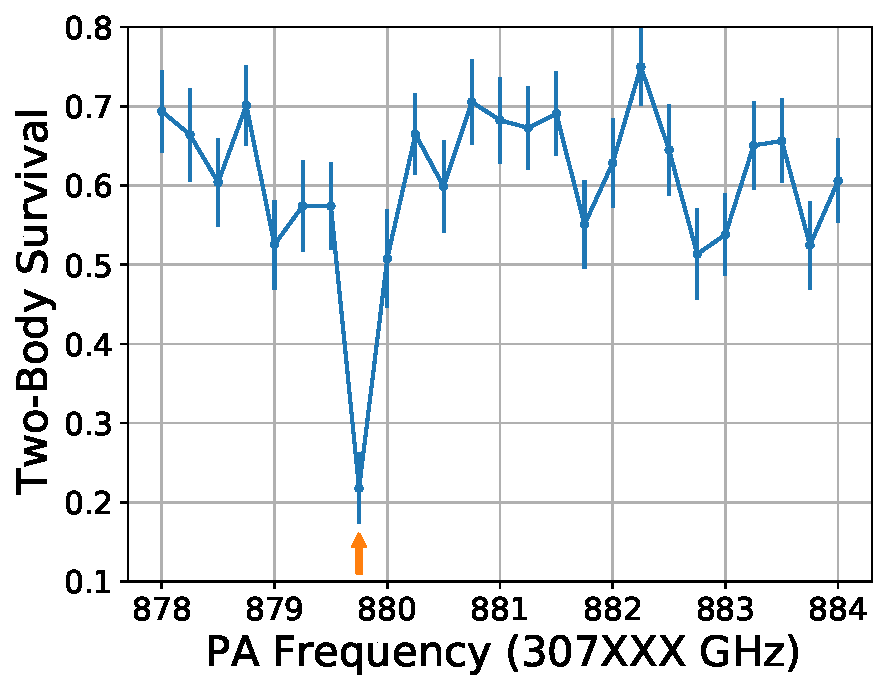
\includegraphics[height=4.5cm]{pa_spectrum_v13.pdf}};
  \node at (2.55, -2.7) {\scriptsize (\textbf{C})};
  \node at (6, -4.6) {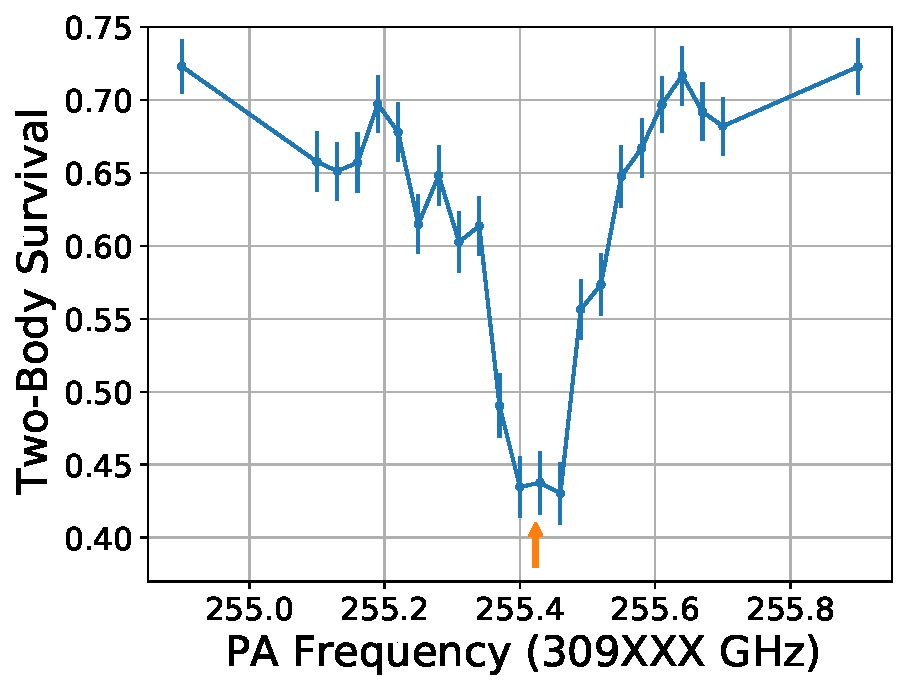
\includegraphics[height=4.5cm]{pa_spectrum_v14.pdf}};
  \node at (8.6, -3.2) {\scriptsize (\textbf{D})};
\end{tikzpicture}
\end{document}
